\documentclass[11,leqno,fleqn]{scrbook}
\usepackage[utf8]{inputenc}
\usepackage[german]{babel}
\usepackage{amsmath}
\usepackage{amsthm}
\usepackage{graphicx}
\usepackage{tabularx}
\usepackage{tcolorbox}
\usepackage{tikz}
\usepackage{wrapfig}
\usepackage{hyperref}


\graphicspath{{figures/}}

\setlength{\parindent}{0mm}

\newtheoremstyle{DefinitionsAndTheorems}{7pt}{3pt}{}{}{\bfseries}{}{\newline}{\thmname{#1} \thmnumber{#2}: \thmnote{#3.}}
\theoremstyle{DefinitionsAndTheorems}
\newtheorem{definition}{Definition}[section]
\newtheorem{theorem}{Satz}[section]

\newtheoremstyle{ExamplesAndExercises}{7pt}{3pt}{}{}{\bfseries}{}{ }{\thmname{#1} \thmnumber{#2} \thmnote{(#3)}}
\theoremstyle{ExamplesAndExercises}
\newtheorem{xmpl}{Beispiel}[chapter] % Dies wird unten mit newenvironment umgedeutet zwecks Kreis als Schlusssymbol
\newtheorem{exercise}{Übung}[section]

% Siehe newtheorem xmpl ohne Kreis als Schlusssymbol
\newenvironment{example}[1]{\begin{xmpl}#1}{\hfill $^\bigcirc$ \end{xmpl}}

% Beweis-Umgebung mit q.e.d.-Box und ohne Eingabe von "Beweis"; heisst prove, da proof reserviert;
\newenvironment{prove}{\begin{proof}[Beweis]}{\end{proof}}

% Lernzielumgebung
\newenvironment{lernziele}{\subsubsection*{Lernziele}\begin{itemize}}{\end{itemize}}

%***********
%\includeonly{}
%***********

\title{Mathematik I}
\author{\copyright Mathias Bosshardt und Franziska Flegel}
\date{Herbst 2024}

\begin{document}
\maketitle

\frontmatter
\tableofcontents  %\listoftables  \listoffigures

\mainmatter
\chapter{Einführung}

\section{Was ist Mathematik?}
\begin{wrapfigure}{r}{0.45\textwidth}
    \vspace{-.8cm}
	\begin{center}
		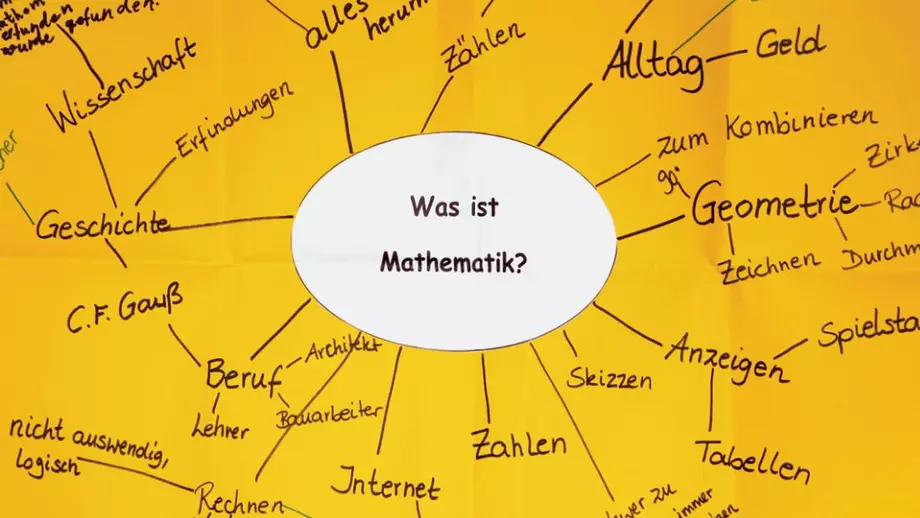
\includegraphics[width=0.96\linewidth]{WasIstMathematik}
	\end{center}
\end{wrapfigure}
Mathematik ist keine Naturwissenschaft. Sie hat aber dennoch viele Anwendungen in den Naturwissenschaften, insbesondere in der Physik, aber auch in anderen Disziplinen, wie etwa den Ingenieur- oder Wirtschaftswissenschaften.
Mathematik beschäftigt sich damit, Muster und Strukturen zu erkennen. 
Sie vermittelt keine interpretationsbedürftigen Ansichten.
Sie baut auf objektiven Sachverhalten und logischen Schlussfolgerungen auf.\par

\section{Warum Mathematik?}
Durch Mathematik können wir viele Dinge in der Welt besser verstehen und begründete Zukunftsprognosen abgeben.
Mathematik ist ein Teil unserer Kultur und zugleich die Antwort des Menschen auf die Komplexität der Welt.
Uns ist oft nicht bewusst, wie
\begin{wrapfigure}{l}{0.5\textwidth}
    \vspace{-.4cm}
	\begin{center}
		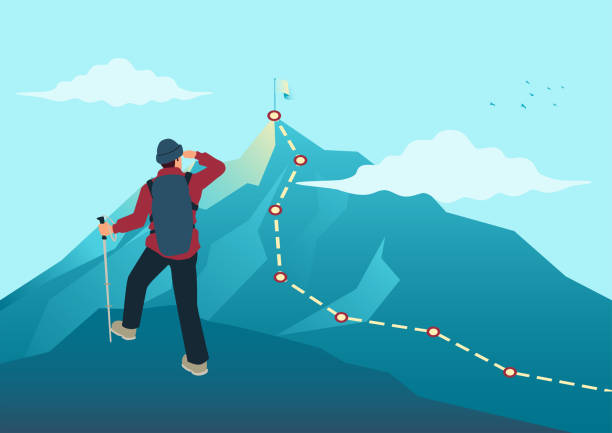
\includegraphics[width=0.96\linewidth]{Bergsteigen}
	\end{center}
	\caption{Der Weg ist das Ziel.}
\end{wrapfigure}
sehr unser Alltag mit Mathematik durchsetzt ist.
Mathematik steckt im Mobiltelefon, im Auto, in stabilen Gebäuden, in medizinischen Untersuchungsmethoden, in CDs, in der kühlen Cola, die du trinkst, wenn es dir mal wieder zu heiss wird\ldots
Mathematisches Können erwirbt man aber nur durch mathematisches Tun. Wer in der Mathematik voran kommen will, muss üben, sich mit der Materie auseinandersetzen. Bergsteigen lernt man ja auch nicht, indem man Bücher über Berge liest.
Wer die Aussicht auf dem Gipfel geniessen will, muss sich anstrengen, muss sich der Aufgabe stellen und selber auf den Berg steigen.
Genauso lassen sich die Schönheit und Harmonie der Mathematik nur erkennen, wenn man sich mit ihr beschäftigt.

\begin{figure}
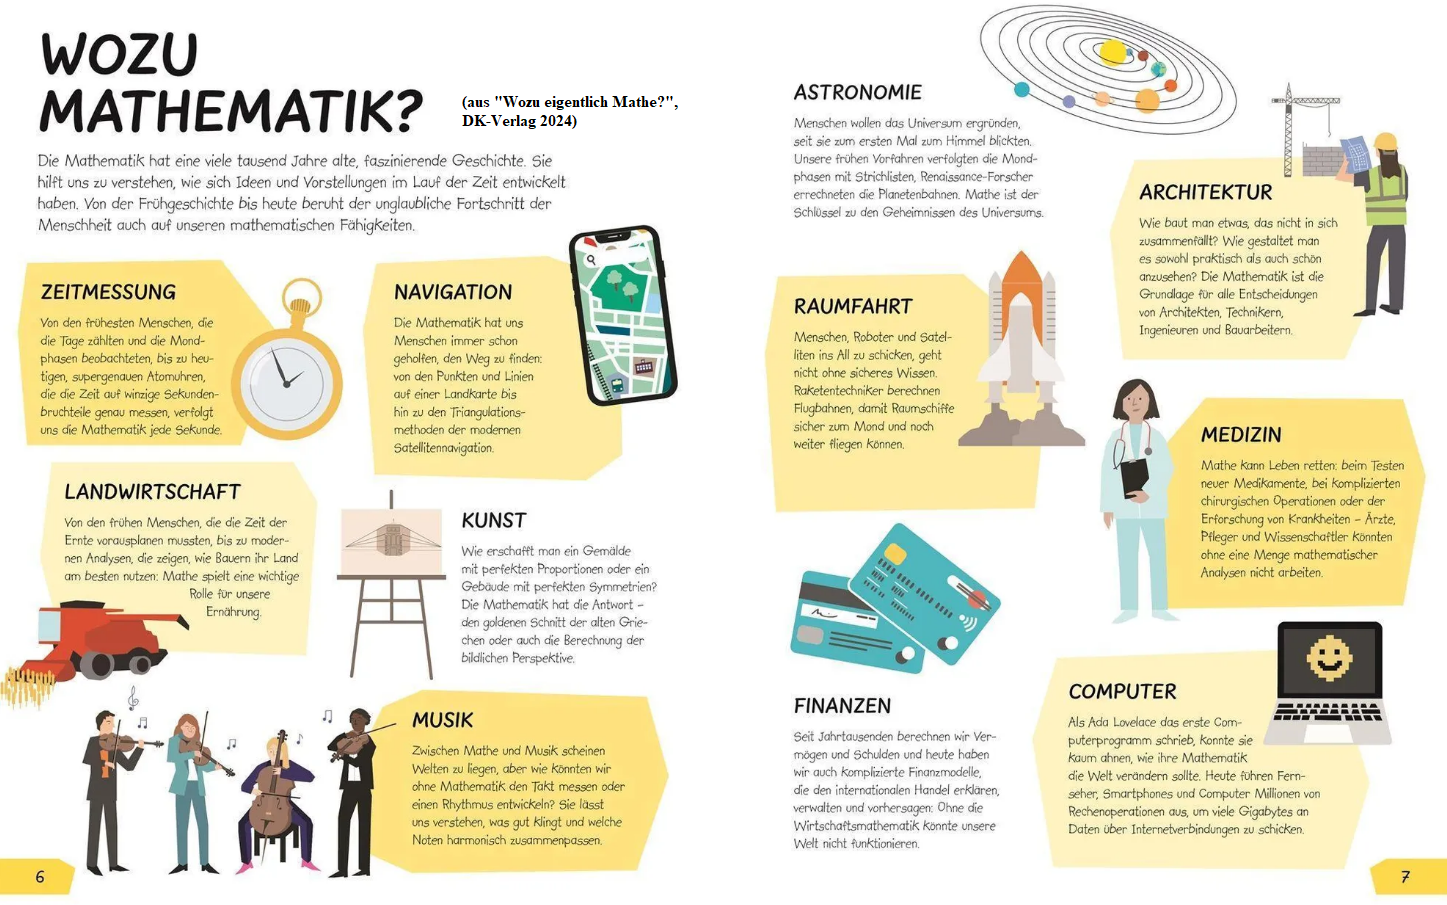
\includegraphics[angle=90,scale=0.6]{WozuMathematik}
\end{figure}
\thispagestyle{empty}

\chapter{Brückenkapitel (0)}
Im ersten Kapitel, oder eher im nullten gemäss Aufgabenbuch, repetieren wir einige Dinge, die ihr auf der Oberstufe gelernt habt.
Damit sind wir dann alle auf dem gleichen Stand.
Und teilweise erweitern wir unser Wissen bereits etwas, führen vielleicht neue Schreibweisen ein, formulieren die Rechengesetze evtl. etwas allgemeiner oder manchmal abstrakter, als du es bisher gewohnt warst. Vielleicht ist das für dich zum grössten Teil ein alter Hut - aber Übung macht den Meister!

\section{Rechnen mit Zahlen -- Die Rechengesetze}
Ein Gesetz ist bekanntermaßen eine feste Regel oder eine verbindliche Vorschrift.
An ihm darf man nichts rütteln oder verschieben, sondern man muss sich daran halten.
Genauso, wie es in den Gesetzbüchern Gesetze gibt, gibt es auch in der Mathematik Regeln, die gelten und beim Rechnen eingehalten werden müssen.
Diese sind die Rechengesetze oder Rechenregeln.
\begin{center}
\begin{tcolorbox}[colback=green!10!white,colframe=green!70!black,title=Rechengesetz,width=.9\linewidth]
		Ein Rechengesetz ist eine verbindliche Rechenvorschrift.
\end{tcolorbox}
\end{center}
Wenn du ein Rechengesetz missachtest, bekommst du natürlich keine Strafe von der Polizei.
Aber wenn du dich nicht an die Rechengesetze hältst, dann wird dein Ergebnis mit grosser Wahrscheinlichkeit falsch sein.
Die Rechengesetze gibt es also nicht, um verzweifelte Schüler:innen zu quälen, sondern sie ergeben mathematisch und logisch Sinn.

Wenn man von den Rechengesetzen spricht, dann meint man meistens das Assoziativgesetz, das Kommutativgesetz und das Distributivgesetz.
Sie sind die drei wichtigsten Rechengesetze.Wenn man den Begriff aber etwas weiter fasst, gibt es noch einige weitere Rechenregeln.
Diese sind etwa die Regel Punkt-vor-Strich, die Potenzgesetze und die Wurzelgesetze, oder Vorgehensweisen zum Auflösen von Klammern.
Fangen wir also an.

\subsection{Rechengesetze}

\begin{center}
\begin{tcolorbox}[colback=red!10!white,colframe=red!70!black,title=Rechengesetze,width=.97\linewidth]
	\begin{enumerate}
        \item
			Kommen Potenzen vor, müssen diese als erstes berechnet werden.
		\item
			Klammern in Termen müssen zuerst aufgelöst werden. ("`von innen nach aussen"')
        \item
			Punktrechnungen ( $\cdot$ und : ) müssen vor Strichrechnungen ( + und -- ) ausgeführt werden.
		\item
			Assoziativgesetz der Addition:\\
			Für alle rellen Zahlen $a$, $b$ und $c$ gilt: $(a+b)+c = a+(b+c)$
		\item
			Assoziativgesetz der Multiplikation:\\
			Für alle rellen Zahlen $a$, $b$ und $c$ gilt: $(a\cdot b)\cdot c = a\cdot (b\cdot c)$
		\item
			Kommutativgesetz der Addition:\\
			Für alle rellen Zahlen $a$ und $b$ gilt: $a+ b= b+ a$
		\item
			Kommutativgesetz der Multiplikation:\\
			Für alle rellen Zahlen $a$ und $b$ gilt: $a\cdot b= b\cdot a$
		\item
			Distributivgesetz der Multiplikation:\\
			Für alle rellen Zahlen $a$, $b$ und $c$ gilt: $(a\pm b)\cdot c = a\cdot c \pm b\cdot c$
		\item
			Distributivgesetz der Division:\\
			Für alle rellen Zahlen $a$, $b$ und $c$ gilt: $(a\pm b): c = a: c \pm b: c$	
	\end{enumerate}
\end{tcolorbox}
\end{center}

\begin{example}
Im folgenden Term darf nicht einfach von links nach rechts gerechnet werden, sondern es muss zuerst das Produkt berechnet werden:
\[
	5+5\cdot 3
\]
\end{example}

\begin{example}
Berechne den folgenden Term:
\[
	4\cdot(27-(3\cdot (5+3)+2))
\]
\end{example}

\begin{example}
Rechne vorteilhaft:
\[
	85+33+67
\]
\end{example}

\begin{example}
Rechne vorteilhaft:
\[
	7\cdot 4 \cdot 45
\]
\end{example}

\begin{example}
Ebenso:
\[
	24+33+76
\]
\end{example}

\begin{example}
Multipliziere aus:
\[
	4\cdot (20-5)
\]
\end{example}

\begin{example}
Manchmal bringt ausklammern einen Vorteil!
\[
	14\cdot 13 - 4\cdot 13
\]
\end{example}

\begin{tcolorbox}[colback=green!10!white,colframe=green!70!black,title=Betrag einer Zahl,width=.9\linewidth]
		Für eine Zahl $a$ ist der Betrag der Zahl
		\[
			|a|=\left\{\begin{array}{ll} a, & a\ge 0 \\
         -a, & a<0\end{array}\right.
		\]
\end{tcolorbox}


\section{Terme}
\subsection*{Auswerten}
Mit $T(a,b)$ bezeichnen wir einen Term, der die Variablen $a$ und $b$ enthält. Setzt man anstelle von $a$ und $b$ Zahlen ein, z.B. 5 für $a$ und 3 für $b$, so schreiben wir $T(5,3)$.
\vspace{1cm}

\subsection*{Termumformungen}
Zwei Terme $T_1$ und $T_2$ heissen \emph{äquivalent (gleichwertig)}, wenn alle möglichen Einsetzungen für die Variable(n) bei $T_1$ denselben Wert ergeben wie bei $T_2$.
Man schreibt: $T_1 = T_2$.
\vspace{5mm}
Einen Term umformen bedeutet:
Man ersetzt ihn durch einen äquivalenten Term. Beim Umformen von Termen werden die arithmetischen Grundgesetze gebraucht.

\begin{tcolorbox}[colback=red!7!white,colframe=red!60!black,title=Arithmetische Grundgesetze]
    \bgroup
    \def\arraystretch{2.5}
	\begin{tabularx}{\linewidth}{|X|c|c|}
			\hline
			 & Addition & Multiplikation \\
			\hline
			Kommutativgesetz & $a+b=b+a$ & $a\cdot b = b\cdot a$ \\
			
			Assoziativgesetz & $(a+b)+c = a+ (b+c)$ & $(a\cdot b)\cdot c = a\cdot (b\cdot c)$ \\
			
			Neutralelement 0 bzw. 1 & $a+0 = a$ & $a\cdot 1 = a$ \\
			
			Inverses Element $-a$ bzw. $\displaystyle \frac{1}{a}$ & $a+(-a) = 0$ & $\displaystyle a\cdot \frac{1}{a} = 1$ \\
			\hline
			Distributivgesetz & \multicolumn{2}{c|}{$a(b+c)=ab+ac$} \\
			\hline
    \end{tabularx}
    \egroup
\end{tcolorbox}

\subsection*{Formeln}
Die \emph{Binomischen Formeln} benutzt man zum schnellen Umformen von Produkten aus Binomen.
Sie stellen Merkformeln dar, die einerseits das Ausmultiplizieren von Klammerausdrücken erleichtern, andererseits aber auch die Faktorisierung von Termen (Umformung von bestimmten Summen und Differenzen in Produkte) erlauben.

\begin{tcolorbox}[colback=blue!7!white,colframe=blue!60!black,title=Binomische Formeln]
	\begin{tabbing}
		$(a+b)^2$ \qquad \, \, \= $=$ \, \= $a^2+2ab+b^2$ \\
		$(a-b)^2$ \qquad \, \, \= $=$ \, \= $a^2-2ab+b^2$ \\
		$(a+b)(a-b)$ \> $=$ \> $a^2-b^2$
	\end{tabbing}
\end{tcolorbox} 

Es gibt auch trinomische Formeln: $(a+b+c)^2$. Kannst du dafür auch einen Ausdruck angeben?
\vspace{2cm}

\subsection*{Erweiterung}
Mit dem \emph{Pascalschen Dreieck} kann man auch höhere Potenzen von Binomen schnell ausmultiplizieren:
\[
	(a+b)^3 =
\]







\end{document} 
